\chapter[Resultados da Mineração]{RESULTADOS DA MINERAÇÃO}

Este capítulo apresenta os resultados da Etapa 5 do processo KDD. Primeiro é discutido o agrupamento, o caso-limite com 0\% de rótulos, e em seguida a classificação semi-supervisionada com taxas de rotulagem de 5\% a 70\%.

\section{AGRUPAMENTO: O CASO-LIMITE COM 0\% DE RÓTULOS}

\subsection{ESCOLHA DO NÚMERO DE GRUPOS NO K-MÉDIAS}

Para verificar se a estrutura dos dados sugere, por si só, o número de classes, o K-Médias foi executado com $k$ de 2 a 10, registrando a inércia (método do cotovelo) e a silhueta. A silhueta, que não usa rótulos, atinge o máximo exatamente no número real de classes nas duas bases: $k = 2$ no Breast Cancer (silhueta de 0,349) e $k = 3$ no Wine (0,288), como mostra a Figura \ref{fig:kmeans_k_wine} para o Wine.

\begin{figure}[htbp]
    \centering
    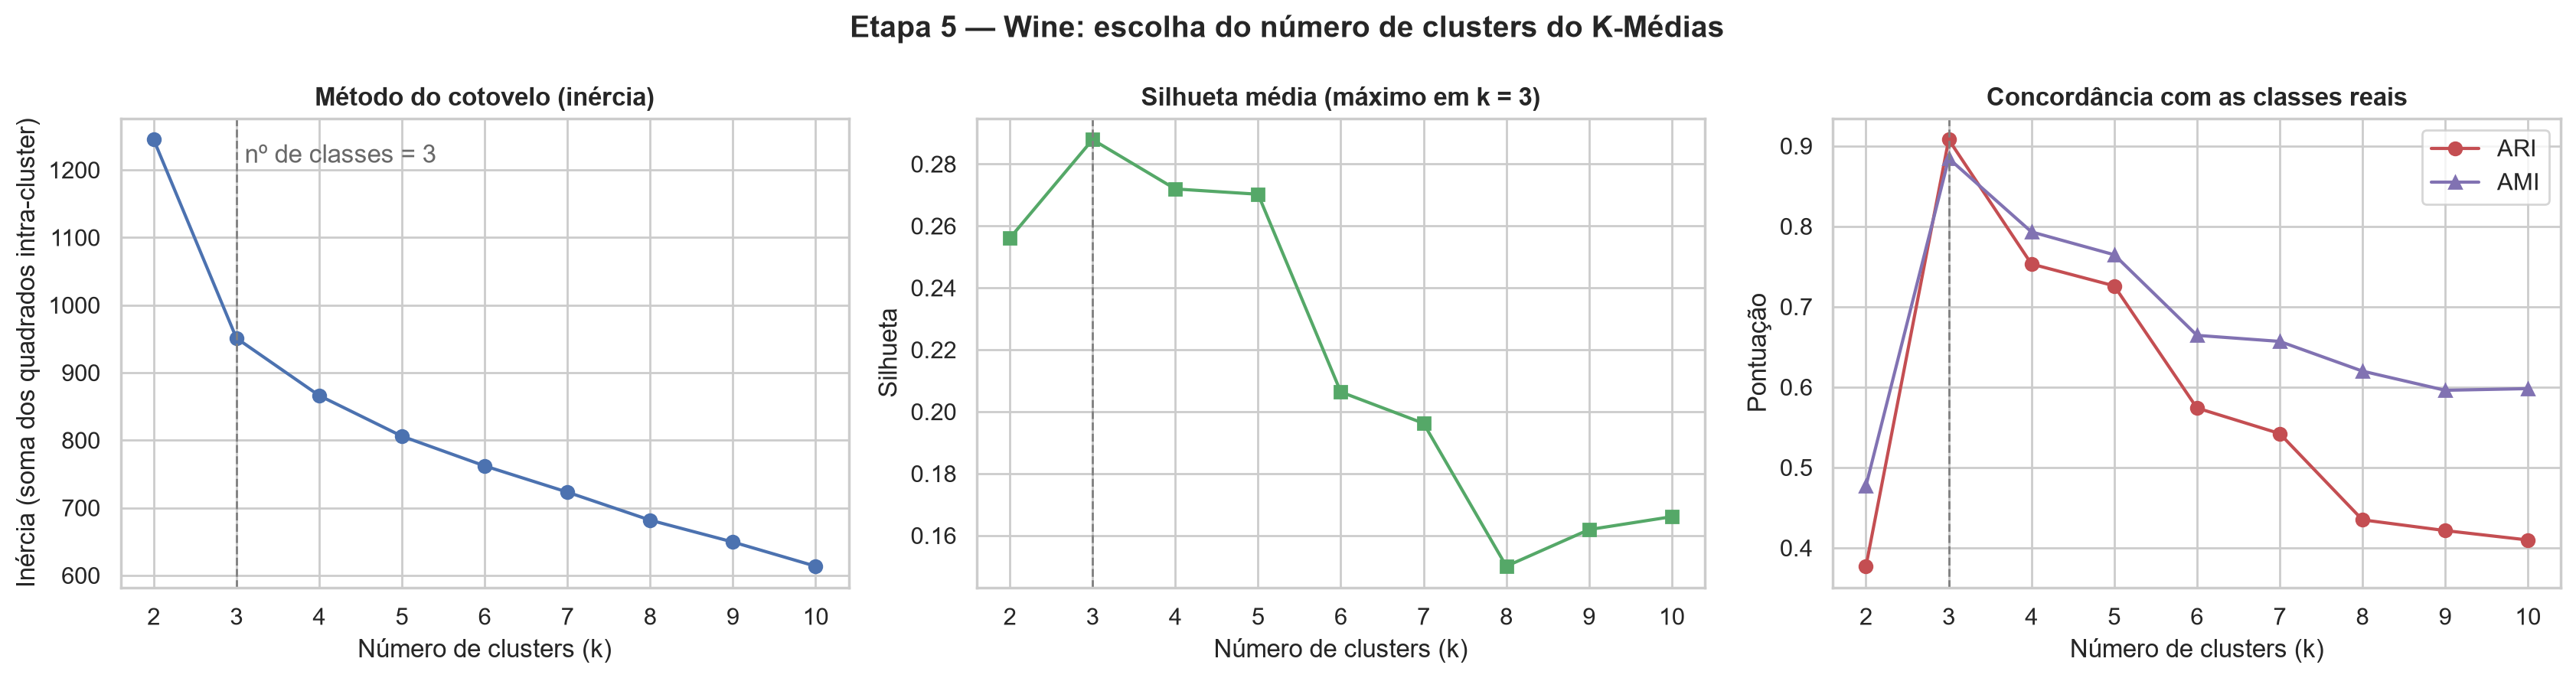
\includegraphics[width=\textwidth, keepaspectratio]{figuras/E5_wine_kmeans_escolha_k.png}
    \caption{Wine: inércia, silhueta e concordância com as classes reais (ARI e AMI) do K-Médias em função de $k$.}
    \label{fig:kmeans_k_wine}
\end{figure}

\subsection{K-MÉDIAS E DBSCAN}

A Tabela \ref{tab:agrupamento} resume as métricas de agrupamento com os parâmetros dos \textit{scripts}, e as Figuras \ref{fig:agrupamento_bc} e \ref{fig:agrupamento_wine} mostram os grupos projetados no PCA 2D.

\begin{table}[htbp]
\centering
\caption{Métricas de agrupamento no treino padronizado (0\% rotulado).}
\label{tab:agrupamento}
\begin{tabular}{llccccc}
\toprule
\textbf{Base} & \textbf{Algoritmo} & \textbf{Grupos} & \textbf{Ruído} & \textbf{ARI} & \textbf{NMI} & \textbf{Silhueta} \\
\midrule
\multirow{2}{*}{Breast Cancer} & K-Médias ($k = 2$) & 2 & 0,0\% & 0,672 & 0,555 & 0,349 \\
 & DBSCAN (\texttt{eps} = 4,5) & 1 & 6,1\% & 0,025 & 0,012 & -- \\
\midrule
\multirow{2}{*}{Wine} & K-Médias ($k = 3$) & 3 & 0,0\% & 0,908 & 0,886 & 0,288 \\
 & DBSCAN (\texttt{eps} = 2,3) & 4 & 22,6\% & 0,602 & 0,660 & 0,253 \\
\bottomrule
\end{tabular}
\end{table}

\begin{figure}[htbp]
    \centering
    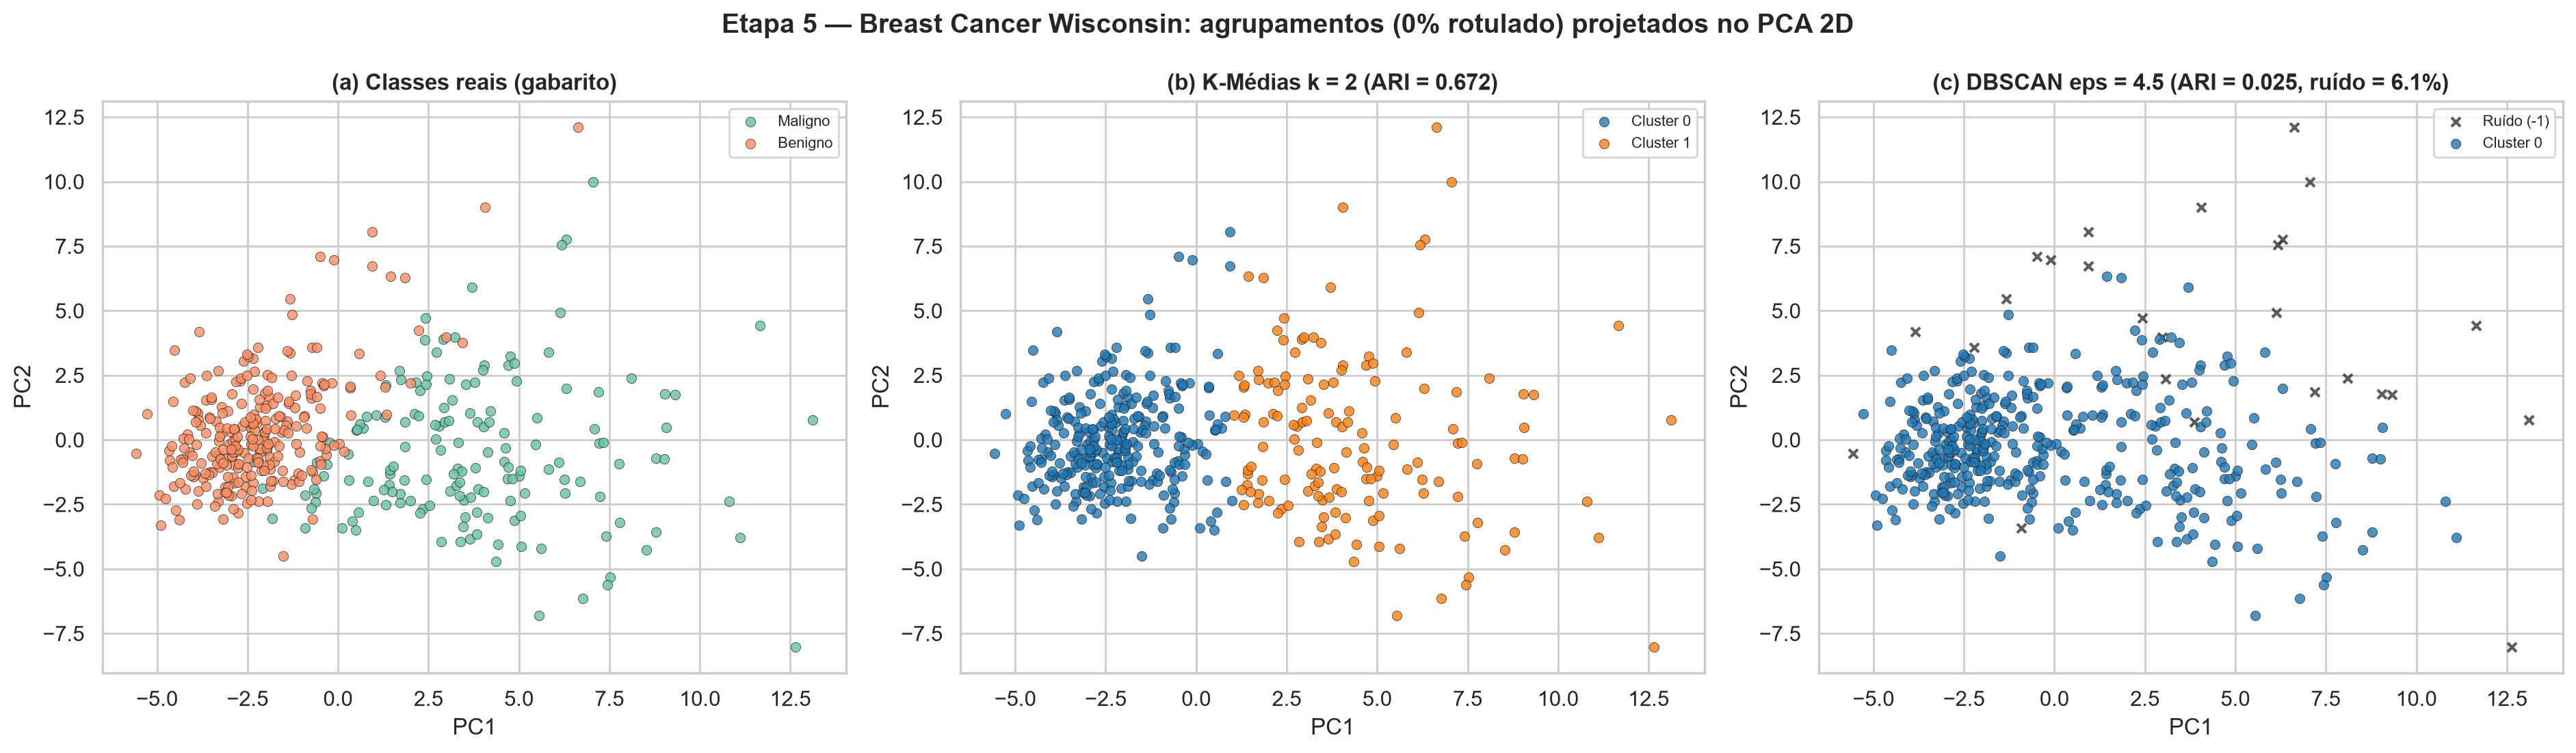
\includegraphics[width=\textwidth, keepaspectratio]{figuras/E5_breast_cancer_agrupamentos_pca.png}
    \caption{Breast Cancer Wisconsin: (a) classes reais, (b) K-Médias e (c) DBSCAN, projetados no PCA 2D.}
    \label{fig:agrupamento_bc}
\end{figure}

No Breast Cancer, os casos benignos formam um grupo compacto, enquanto os malignos se dispersam ao longo da PC1. O K-Médias separa os grupos aproximadamente na mesma fronteira das classes reais (ARI = 0,672). O DBSCAN, por sua vez, une as duas classes em uma massa única e marca como ruído os pontos mais distantes, que são justamente tumores malignos atípicos. O valor de \texttt{eps} do \textit{script} fica próximo ao ``joelho'' da curva de k-distâncias ($\approx$ 4,29). Em uma varredura de 160 combinações de \texttt{eps} e \texttt{min\_samples}, apenas 5 formaram dois ou mais grupos: não existe um ``vale de densidade'' entre benignos e malignos. O melhor ARI da varredura (0,400) foi obtido com um único grupo e 48\% de ruído, ou seja, o DBSCAN só consegue isolar parte da classe maligna como ruído em torno de um núcleo denso. Esse comportamento é coerente com a análise de \textit{outliers} da Etapa 3.

\begin{figure}[htbp]
    \centering
    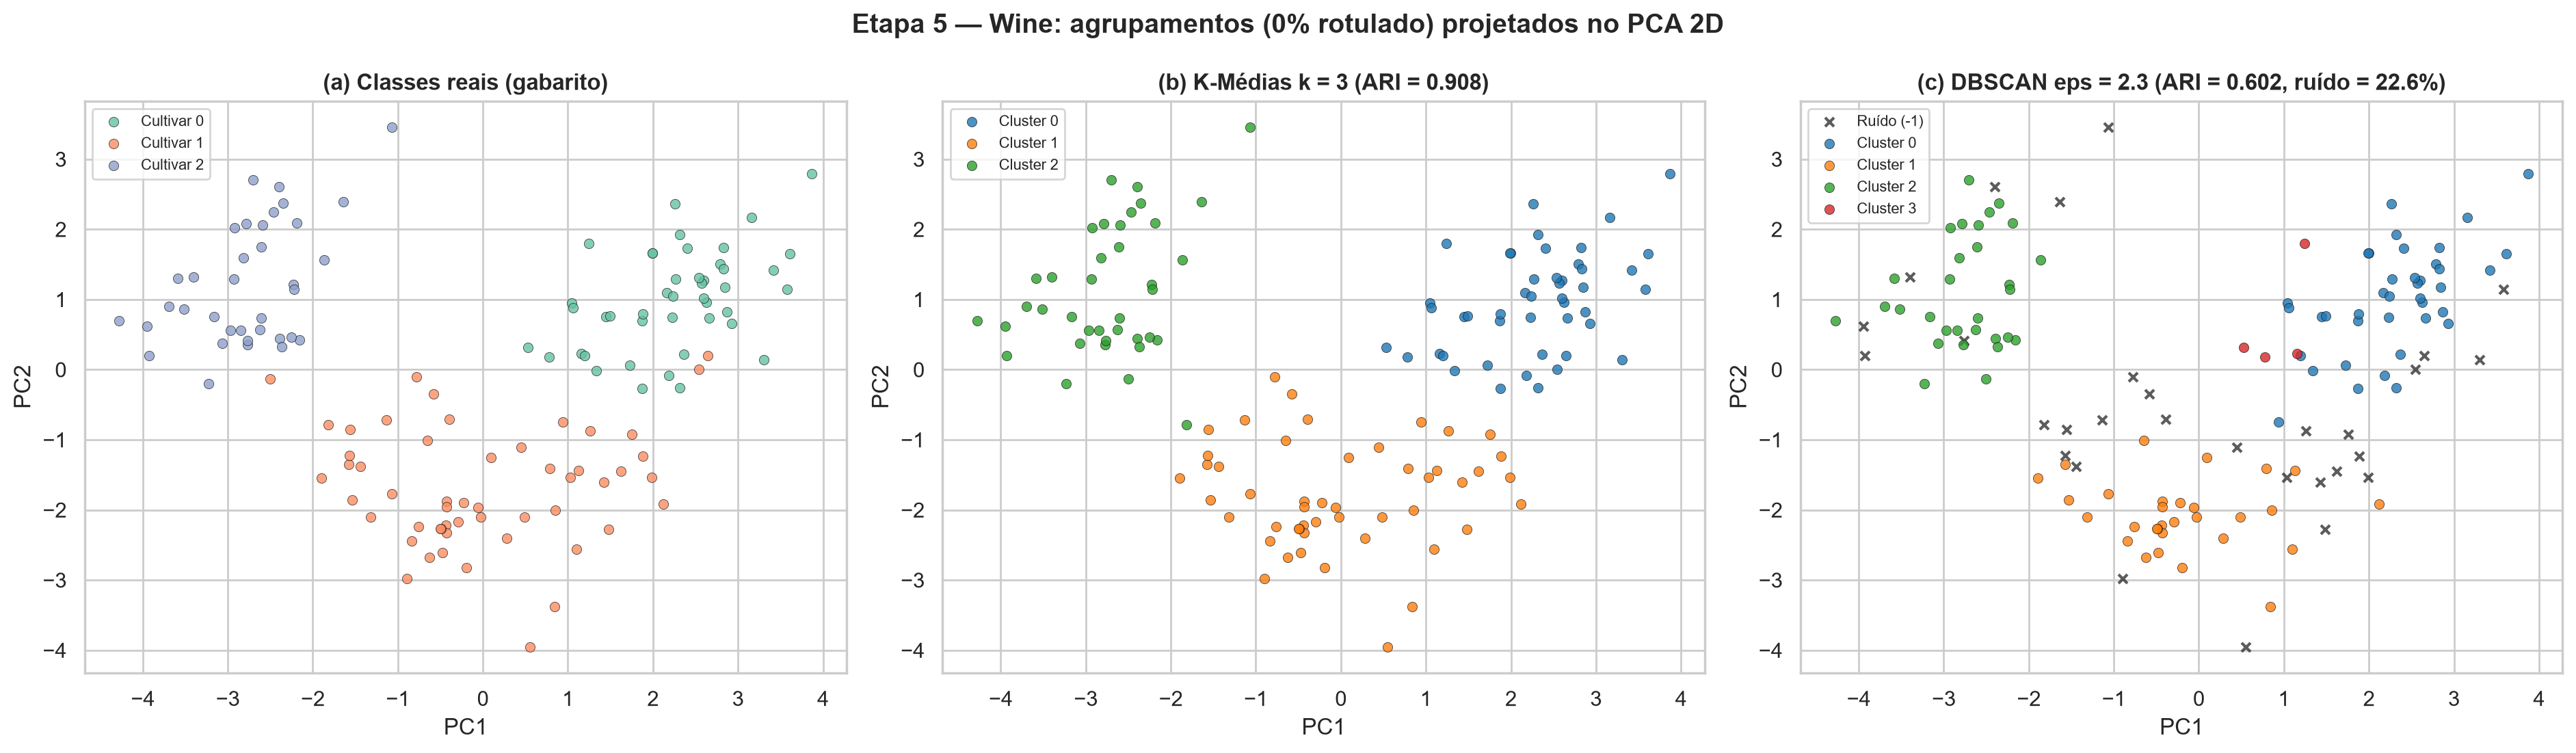
\includegraphics[width=\textwidth, keepaspectratio]{figuras/E5_wine_agrupamentos_pca.png}
    \caption{Wine: (a) classes reais, (b) K-Médias e (c) DBSCAN, projetados no PCA 2D.}
    \label{fig:agrupamento_wine}
\end{figure}

No Wine, as três cultivares formam grupos distintos, com mistura apenas nas faixas de transição, e o K-Médias praticamente reproduz as classes sem nenhum rótulo (ARI = 0,908). O DBSCAN fragmenta a estrutura em quatro grupos e descarta 22,6\% das amostras como ruído, concentrado nas fronteiras entre as cultivares (ARI = 0,602). Esse é o melhor ARI da varredura, mas depende de ajuste fino: com \texttt{min\_samples} = 4, apenas a faixa estreita de \texttt{eps} entre 2,2 e 2,4 separa mais de um grupo, e com \texttt{eps} $\geq$ 2,5, incluindo o joelho da curva ($\approx$ 2,73), tudo se torna um único grupo.

\subsection{DO AGRUPAMENTO AO CLASSIFICADOR}

Para colocar o agrupamento na mesma escala dos classificadores, cada grupo do K-Médias foi associado a uma classe pelo algoritmo húngaro \citep{kuhn1955hungarian}, que encontra a associação um-para-um que maximiza os acertos no treino. Em seguida, os pontos de teste foram atribuídos ao centróide mais próximo. Essa referência é otimista, pois a associação usa os rótulos do treino, mas mostra quanto da estrutura das classes o agrupamento captura sem supervisão: os grupos do K-Médias classificam corretamente \textbf{92,3\%} das amostras de teste no Breast Cancer (F1 = 0,916) e \textbf{95,6\%} no Wine (F1 = 0,956).

Em síntese, após a padronização as classes formam grupos aproximadamente convexos, mas encostados uns nos outros, sem regiões vazias entre elas. Isso favorece o K-Médias e prejudica o DBSCAN. O sucesso do agrupamento no Wine antecipa que os dados não rotulados devem ajudar mais nessa base do que no Breast Cancer.

\section{CLASSIFICAÇÃO SEMI-SUPERVISIONADA}

\subsection{CURVAS DE APRENDIZADO}

As Tabelas \ref{tab:f1_bc} e \ref{tab:f1_wine} e as Figuras \ref{fig:curva_bc} e \ref{fig:curva_wine} apresentam o F1-macro no conjunto de teste em função da taxa de pontos rotulados.

\begin{table}[htbp]
\centering
\caption{Breast Cancer Wisconsin: F1-macro no teste (média $\pm$ desvio padrão em 5 repetições).}
\label{tab:f1_bc}
\footnotesize
\begin{tabular}{ccccc}
\toprule
\textbf{Taxa} & \textbf{KNN} & \textbf{Reg. Logística} & \textbf{Label Spreading} & \textbf{Self-Training LR} \\
\midrule
0,05 & 0,906 $\pm$ 0,014 & 0,926 $\pm$ 0,017 & \textbf{0,936} $\pm$ 0,007 & 0,930 $\pm$ 0,021 \\
0,10 & 0,925 $\pm$ 0,009 & \textbf{0,939} $\pm$ 0,011 & 0,926 $\pm$ 0,011 & 0,936 $\pm$ 0,015 \\
0,20 & 0,942 $\pm$ 0,007 & 0,947 $\pm$ 0,010 & 0,938 $\pm$ 0,014 & \textbf{0,948} $\pm$ 0,007 \\
0,30 & 0,945 $\pm$ 0,017 & \textbf{0,962} $\pm$ 0,012 & 0,944 $\pm$ 0,014 & 0,961 $\pm$ 0,008 \\
0,40 & 0,951 $\pm$ 0,007 & \textbf{0,970} $\pm$ 0,010 & 0,959 $\pm$ 0,012 & 0,965 $\pm$ 0,012 \\
0,50 & 0,956 $\pm$ 0,009 & 0,973 $\pm$ 0,012 & 0,953 $\pm$ 0,014 & \textbf{0,974} $\pm$ 0,009 \\
0,60 & 0,957 $\pm$ 0,007 & \textbf{0,976} $\pm$ 0,006 & 0,956 $\pm$ 0,007 & \textbf{0,976} $\pm$ 0,010 \\
0,70 & 0,964 $\pm$ 0,008 & \textbf{0,982} $\pm$ 0,004 & 0,962 $\pm$ 0,009 & \textbf{0,982} $\pm$ 0,004 \\
\bottomrule
\end{tabular}
\end{table}

\begin{figure}[htbp]
    \centering
    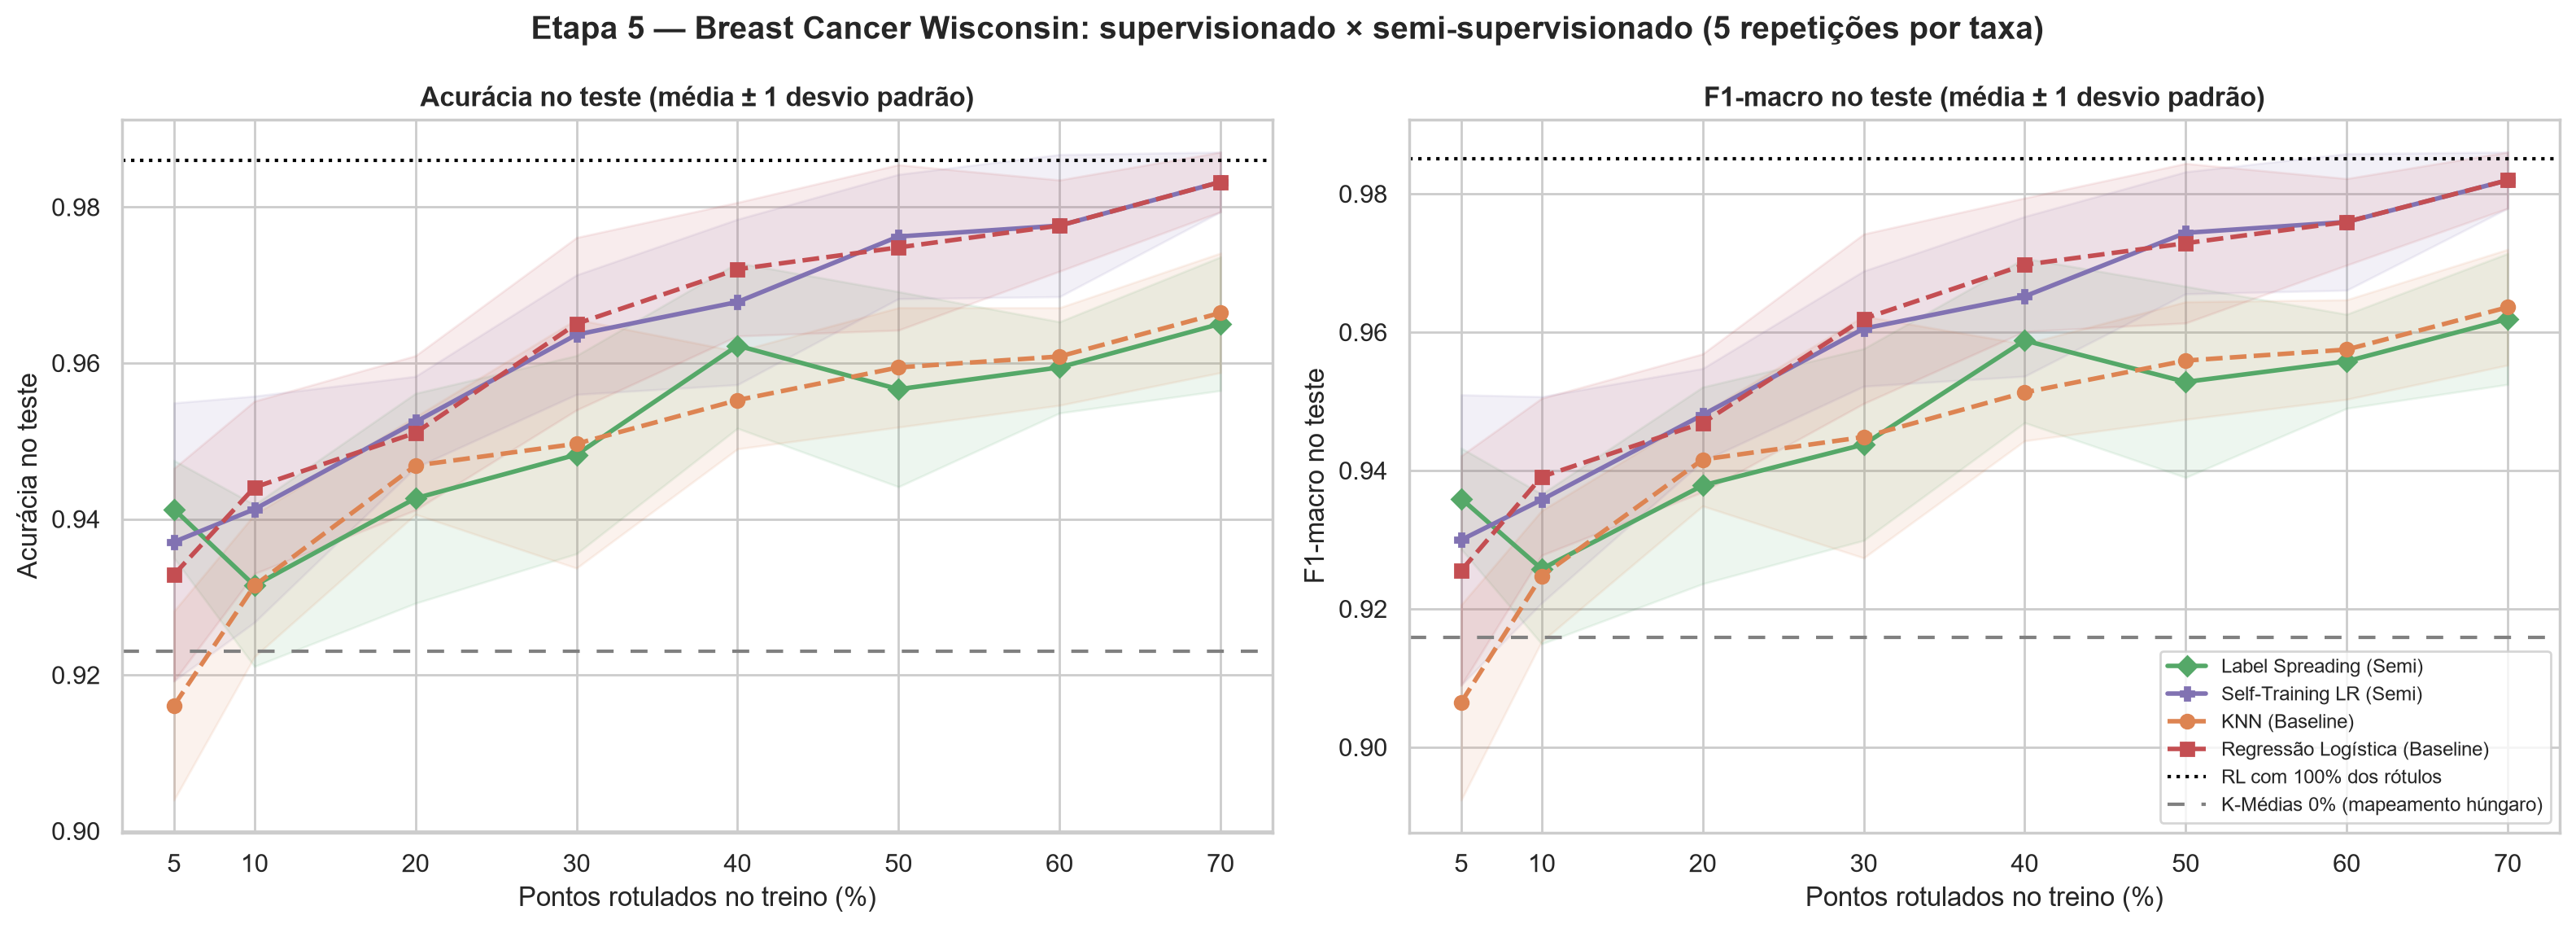
\includegraphics[width=\textwidth, keepaspectratio]{figuras/E5_breast_cancer_curva_aprendizado.png}
    \caption{Breast Cancer Wisconsin: acurácia e F1-macro no teste em função da taxa de rótulos (média $\pm$ 1 desvio padrão).}
    \label{fig:curva_bc}
\end{figure}

No Breast Cancer, com 5\% de rótulos (21 amostras), os métodos semi-\hspace{0pt}supervisionados superam o KNN (de 0,906 para cerca de 0,936), e o \textit{Label Spreading} obtém o maior F1 médio, ligeiramente acima da Regressão Logística (0,936 contra 0,926). As faixas de desvio padrão, no entanto, se sobrepõem, e a partir de 10\% a Regressão Logística já iguala ou supera os métodos semi-supervisionados. Com 70\% dos rótulos, o \textit{Self-Training} e a Regressão Logística produzem exatamente o mesmo F1 (0,982) nas cinco repetições, ou seja, os pseudo-rótulos deixam de alterar as predições no teste. A acurácia média do \textit{Self-Training} considerando todas as taxas de 5\% a 70\% foi de 96,24\%.

\begin{table}[htbp]
\centering
\caption{Wine: F1-macro no teste (média $\pm$ desvio padrão em 10 repetições). Entre parênteses, o número de amostras rotuladas.}
\label{tab:f1_wine}
\footnotesize
\setlength{\tabcolsep}{5pt}
\begin{tabular}{cccccc}
\toprule
\textbf{Taxa} & \textbf{KNN} & \textbf{\shortstack{Reg.\\Logística}} & \textbf{\shortstack{Label\\Spreading}} & \textbf{\shortstack{Label\\Propagation}} & \textbf{\shortstack{Self-Training\\LR}} \\
\midrule
0,05 (7)  & 0,862 $\pm$ 0,091 & 0,930 $\pm$ 0,038 & 0,874 $\pm$ 0,077 & 0,237 $\pm$ 0,089 & \textbf{0,980} $\pm$ 0,013 \\
0,10 (13) & 0,906 $\pm$ 0,040 & 0,937 $\pm$ 0,034 & 0,931 $\pm$ 0,046 & 0,645 $\pm$ 0,227 & \textbf{0,983} $\pm$ 0,017 \\
0,20 (27) & 0,940 $\pm$ 0,025 & 0,971 $\pm$ 0,015 & 0,939 $\pm$ 0,039 & 0,872 $\pm$ 0,072 & \textbf{0,985} $\pm$ 0,010 \\
0,30 (40) & 0,976 $\pm$ 0,012 & 0,969 $\pm$ 0,027 & 0,957 $\pm$ 0,020 & 0,933 $\pm$ 0,018 & \textbf{0,982} $\pm$ 0,018 \\
0,50 (66) & 0,956 $\pm$ 0,018 & 0,973 $\pm$ 0,023 & 0,946 $\pm$ 0,031 & 0,932 $\pm$ 0,028 & \textbf{0,987} $\pm$ 0,016 \\
0,70 (93) & 0,955 $\pm$ 0,018 & 0,986 $\pm$ 0,012 & 0,975 $\pm$ 0,027 & 0,971 $\pm$ 0,030 & \textbf{0,991} $\pm$ 0,012 \\
\bottomrule
\end{tabular}
\end{table}

\begin{figure}[htbp]
    \centering
    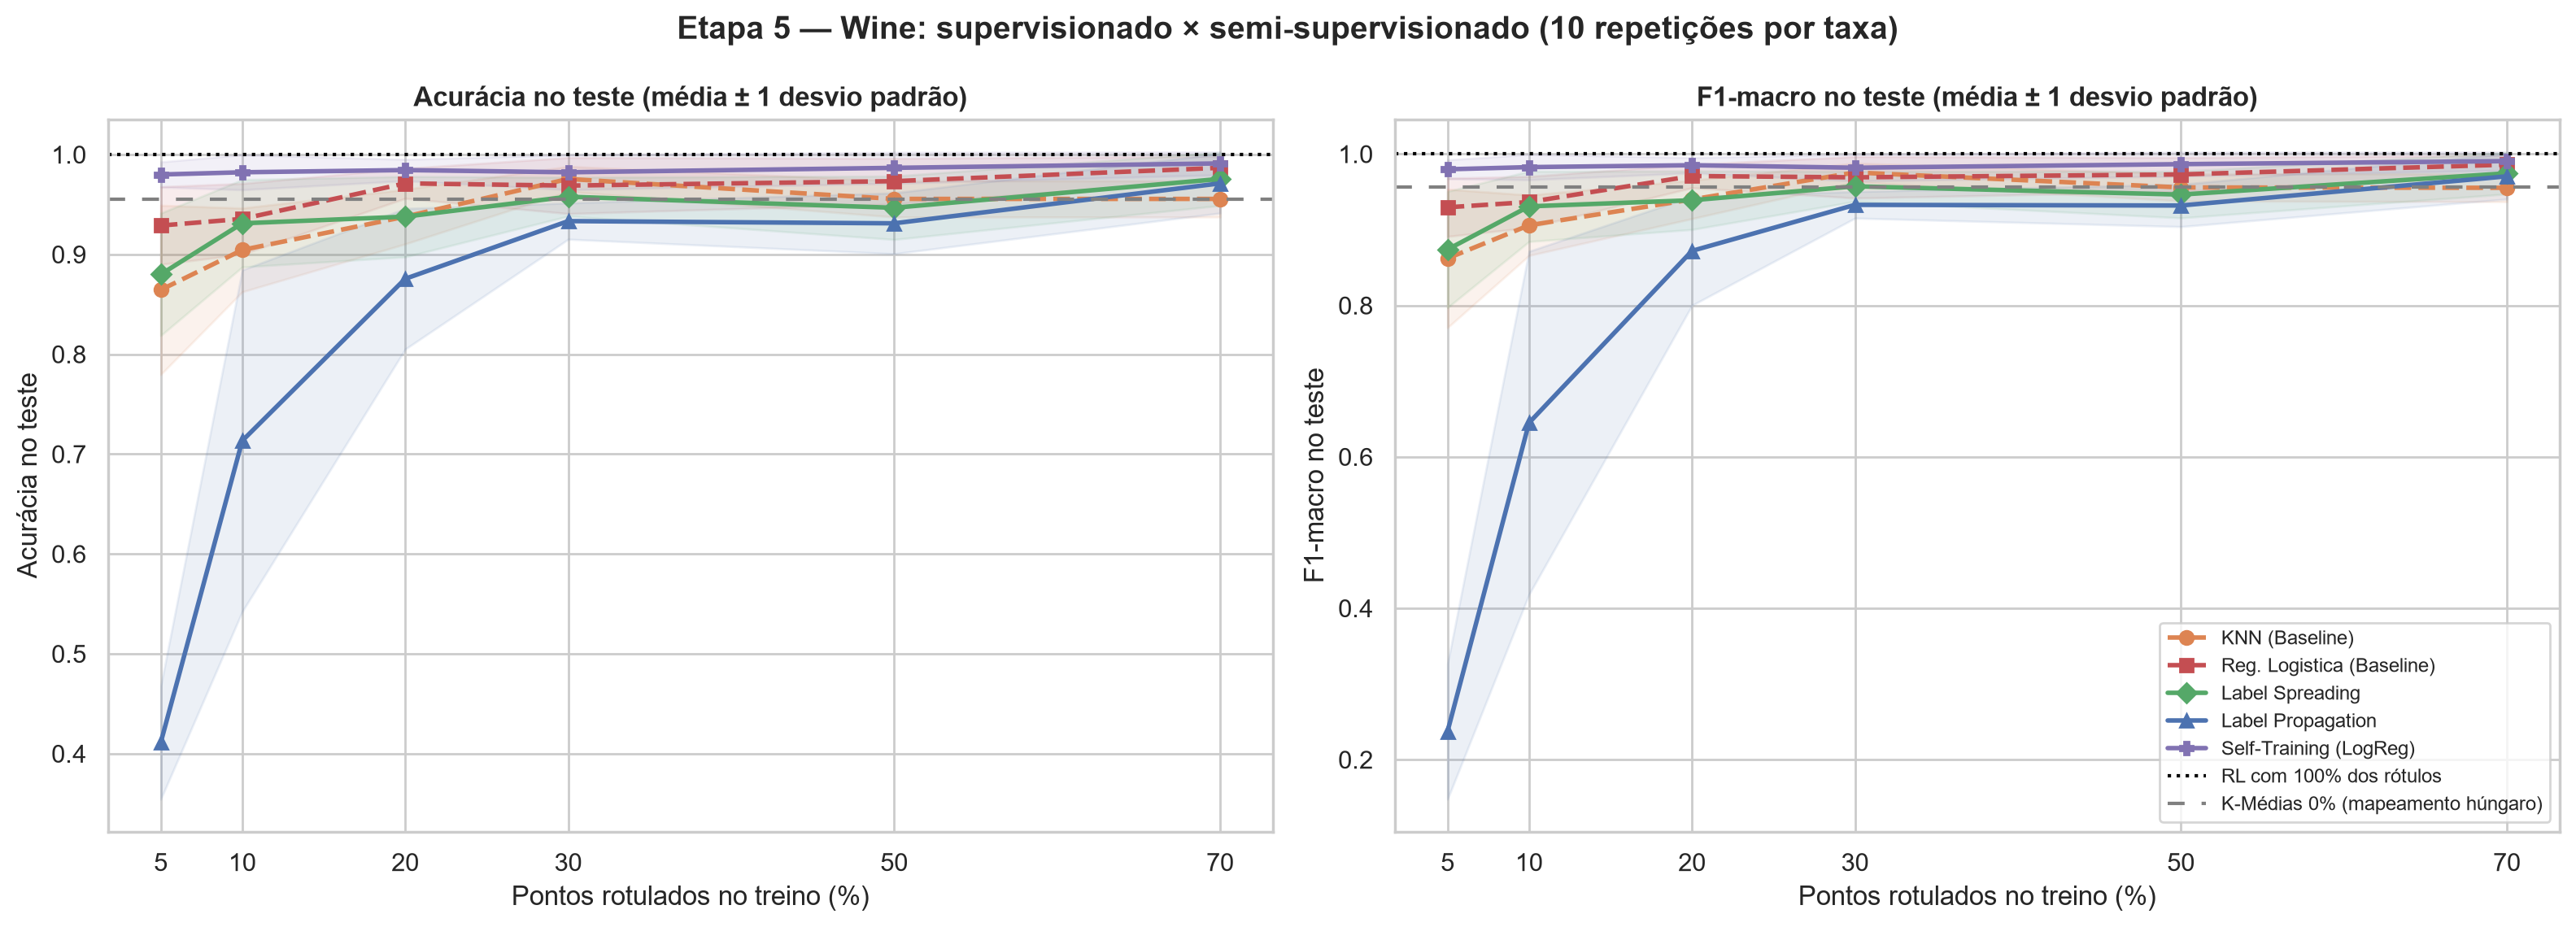
\includegraphics[width=\textwidth, keepaspectratio]{figuras/E5_wine_curva_aprendizado.png}
    \caption{Wine: acurácia e F1-macro no teste em função da taxa de rótulos (média $\pm$ 1 desvio padrão).}
    \label{fig:curva_wine}
\end{figure}

No Wine, o \textit{Self-Training} com Regressão Logística é o melhor método em todas as taxas. Com apenas 7 vinhos rotulados (5\%), atinge F1 = 0,980, contra 0,930 da Regressão Logística e 0,862 do KNN. A acurácia média do \textit{Self-Training} considerando todas as taxas foi de 98,44\%. O \textit{Label Propagation}, por outro lado, colapsa com poucos rótulos (F1 = 0,237 a 5\% e 0,645 a 10\%) e só se recupera a partir de 30\%. Com 70\% dos rótulos, o \textit{Self-Training} e a Regressão Logística convergem para cerca de 0,99.

\subsection{GANHO DO SEMI-SUPERVISIONADO E TESTE DE WILCOXON}

Para cada taxa, o melhor método semi-supervisionado de cada base (o \textit{Self-Training}, que teve o maior F1 médio considerando todas as taxas) foi comparado com cada \textit{baseline} pelo teste de Wilcoxon sobre as repetições pareadas (Figura \ref{fig:wilcoxon} e Tabela \ref{tab:wilcoxon}). É importante observar que, com as 5 repetições do Breast Cancer, o menor p-valor bicaudal possível é $2/2^5 = 0{,}0625$. Portanto, \textbf{nenhuma} diferença nessa base pode ser declarada significativa a 5\%. Com as 10 repetições do Wine, o mínimo é $2/2^{10} \approx 0{,}002$.

\begin{figure}[htbp]
    \centering
    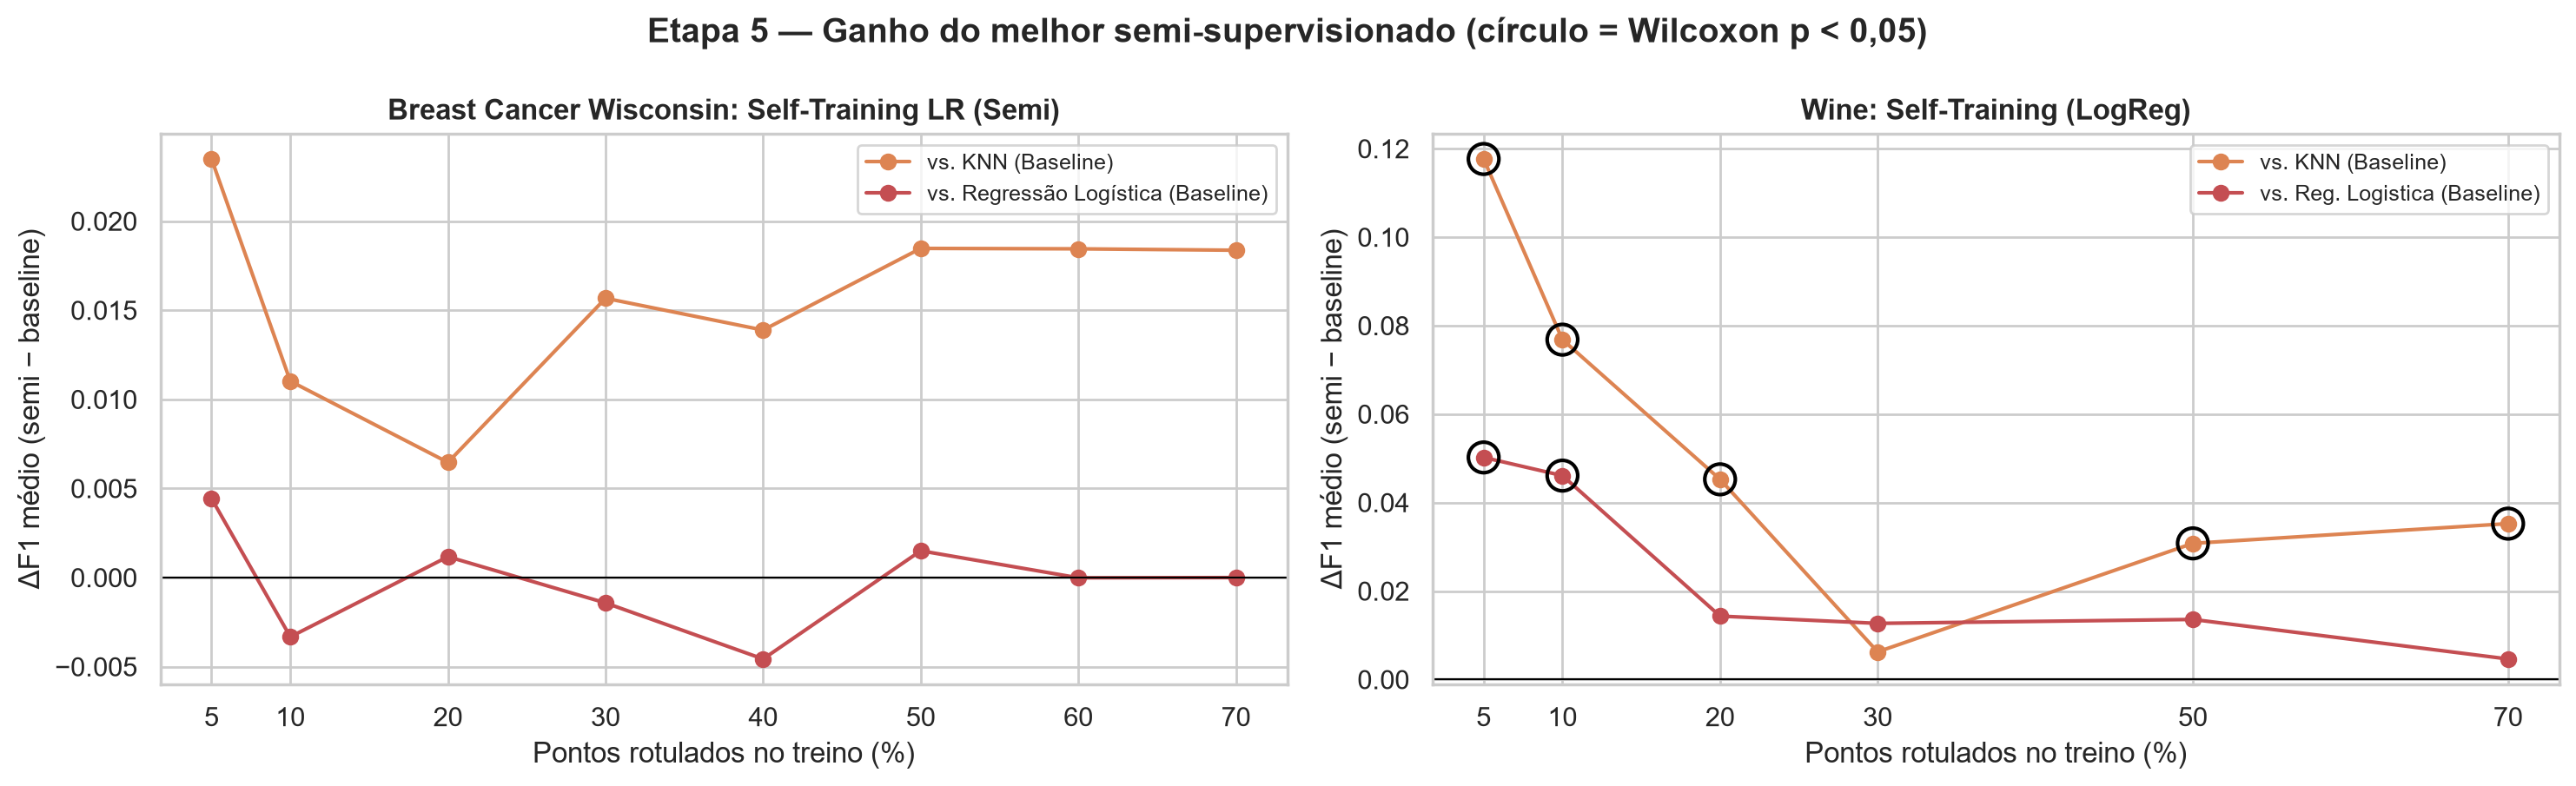
\includegraphics[width=\textwidth, keepaspectratio]{figuras/E5_wilcoxon_ganho.png}
    \caption{Ganho médio de F1-macro do \textit{Self-Training} sobre cada \textit{baseline}. Os círculos indicam diferenças significativas no teste de Wilcoxon ($p < 0{,}05$).}
    \label{fig:wilcoxon}
\end{figure}

\begin{table}[htbp]
\centering
\caption{\textit{Self-Training} LR contra a Regressão Logística nas taxas comuns às duas bases: ganho médio de F1-macro, número de repetições vencidas e p-valor do teste de Wilcoxon.}
\label{tab:wilcoxon}
\footnotesize
\begin{tabular}{ccccccc}
\toprule
 & \multicolumn{3}{c}{\textbf{Breast Cancer (5 repetições)}} & \multicolumn{3}{c}{\textbf{Wine (10 repetições)}} \\
\cmidrule(lr){2-4} \cmidrule(lr){5-7}
\textbf{Taxa} & $\Delta F1$ & \textbf{Vitórias} & \textbf{p} & $\Delta F1$ & \textbf{Vitórias} & \textbf{p} \\
\midrule
0,05 & $+$0,004 & 3/5 & 0,625 & $+$0,050 & 8/10 & \textbf{0,008} \\
0,10 & $-$0,003 & 1/5 & 0,500 & $+$0,046 & 9/10 & \textbf{0,004} \\
0,20 & $+$0,001 & 2/5 & 1,000 & $+$0,014 & 6/10 & 0,094 \\
0,30 & $-$0,001 & 1/5 & 1,000 & $+$0,013 & 5/10 & 0,063 \\
0,50 & $+$0,002 & 2/5 & 0,875 & $+$0,014 & 5/10 & 0,141 \\
0,70 & 0,000 & 0/5 & 1,000 & $+$0,005 & 3/10 & 0,625 \\
\bottomrule
\end{tabular}
\end{table}

No Wine, o \textit{Self-Training} supera a Regressão Logística de forma significativa com 5\% e 10\% de rótulos (ganhos de $+$0,050 e $+$0,046), e supera o KNN de forma significativa em quase todas as taxas. A partir de 20\%, a vantagem sobre a Regressão Logística deixa de ser significativa e diminui até $+$0,005 a 70\%. No Breast Cancer, os ganhos sobre a Regressão Logística oscilam em torno de zero em todas as taxas, e os ganhos sobre o KNN, embora consistentes (o \textit{Self-Training} vence as 5 repetições a partir de 30\%), não podem atingir significância com 5 repetições.

\subsection{MATRIZES DE CONFUSÃO}

As Figuras \ref{fig:matriz_bc} e \ref{fig:matriz_wine} mostram as matrizes de confusão do \textit{Self-Training} em execuções representativas, isto é, na repetição cujo F1 é o mais próximo da média da taxa, com 5\% e 70\% de rótulos.

\begin{figure}[htbp]
    \centering
    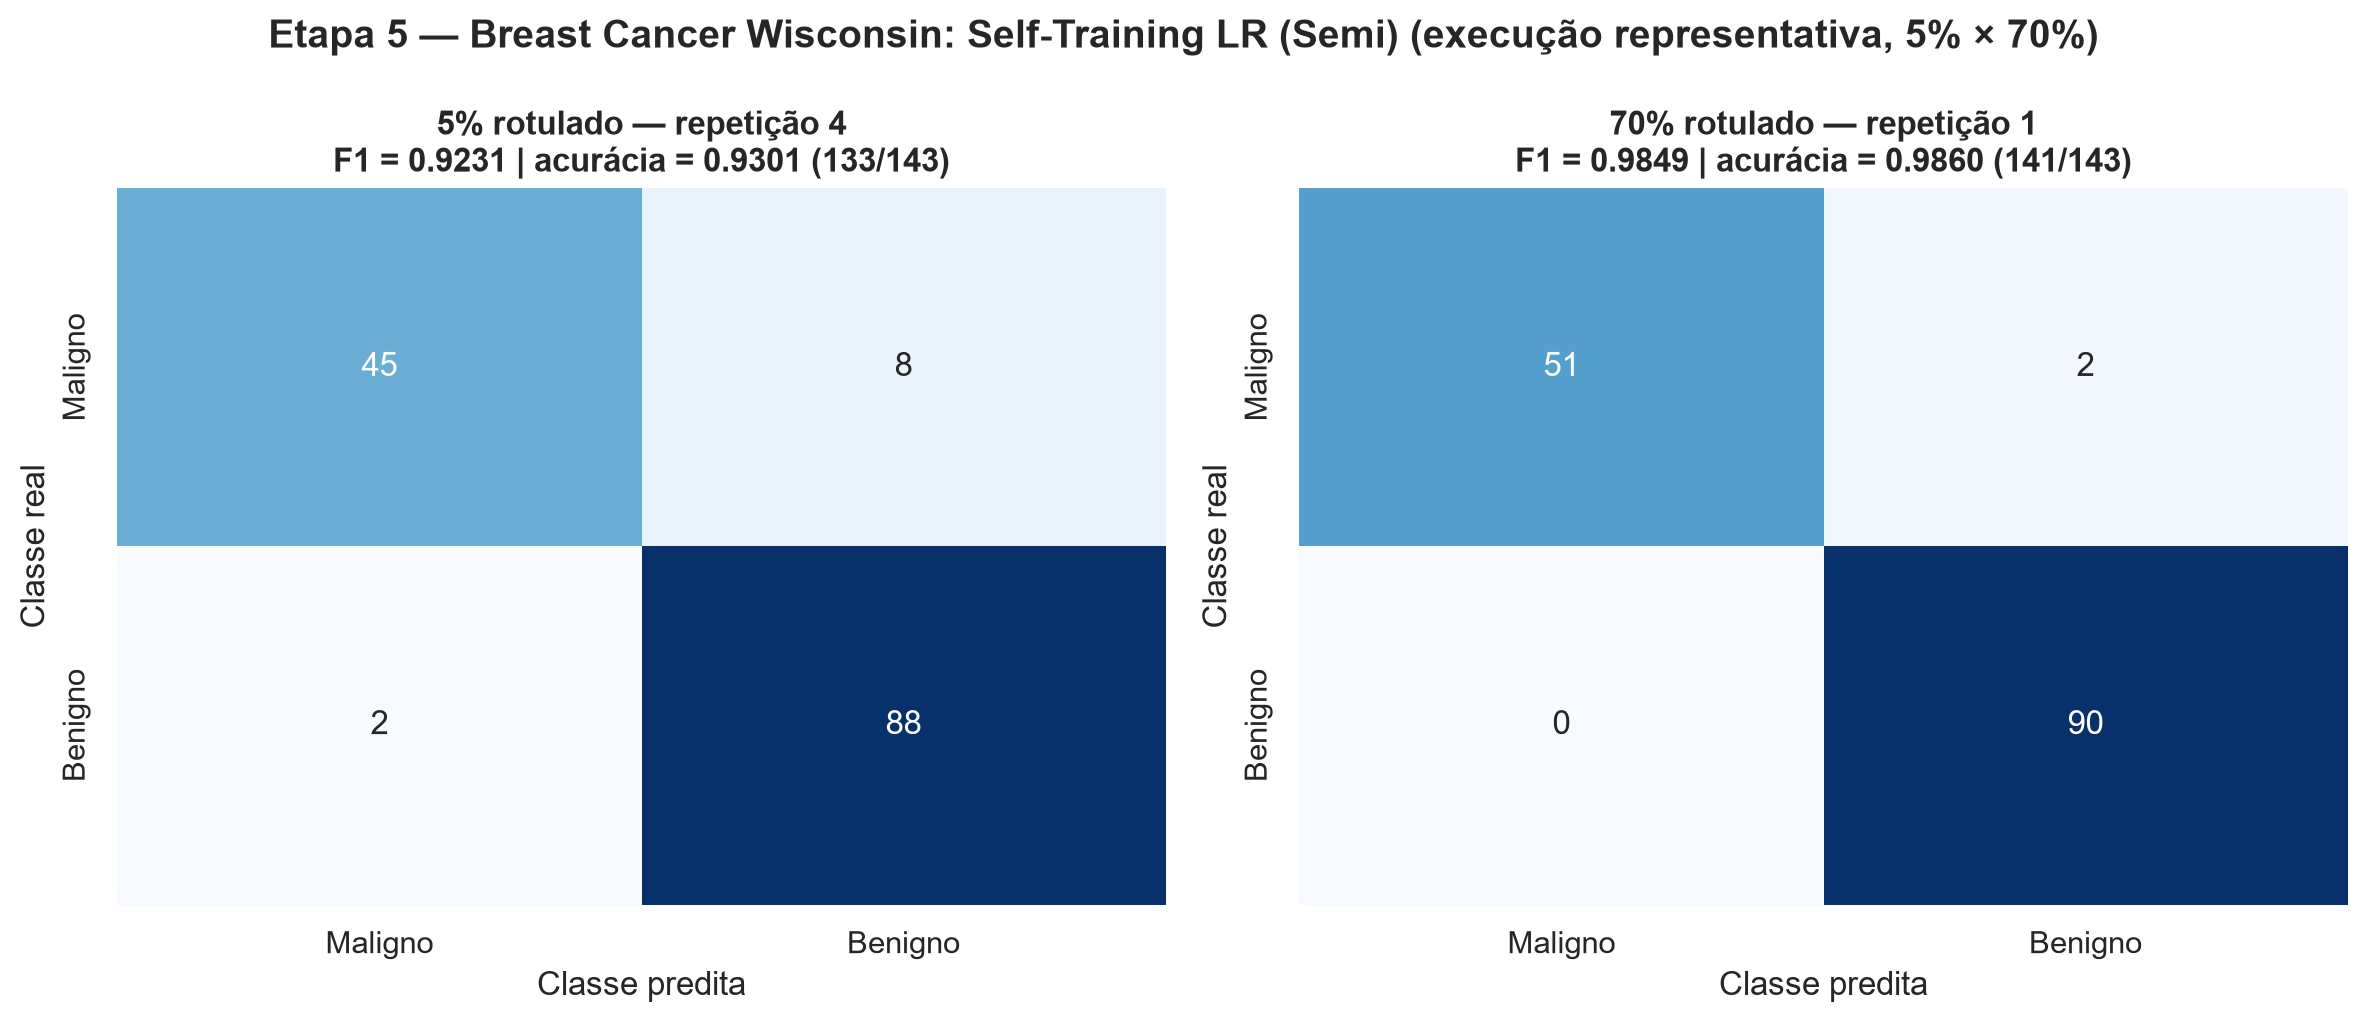
\includegraphics[width=0.9\textwidth, keepaspectratio]{figuras/E5_breast_cancer_matriz_representativa.png}
    \caption{Breast Cancer Wisconsin: matrizes de confusão do \textit{Self-Training} LR com 5\% e 70\% de rótulos (execuções representativas).}
    \label{fig:matriz_bc}
\end{figure}

No Breast Cancer, com 5\% de rótulos, o modelo acerta 133 dos 143 pacientes de teste (93,01\% de acurácia), com 8 falsos negativos e 2 falsos positivos. Com 70\% de rótulos, acerta 141 de 143 (98,60\%), com apenas 2 falsos negativos e nenhum falso positivo. O ganho de 5,59 pontos percentuais corrige 8 diagnósticos incorretos e, principalmente, reduz os falsos negativos, que são o erro mais grave em um contexto de triagem.

\begin{figure}[htbp]
    \centering
    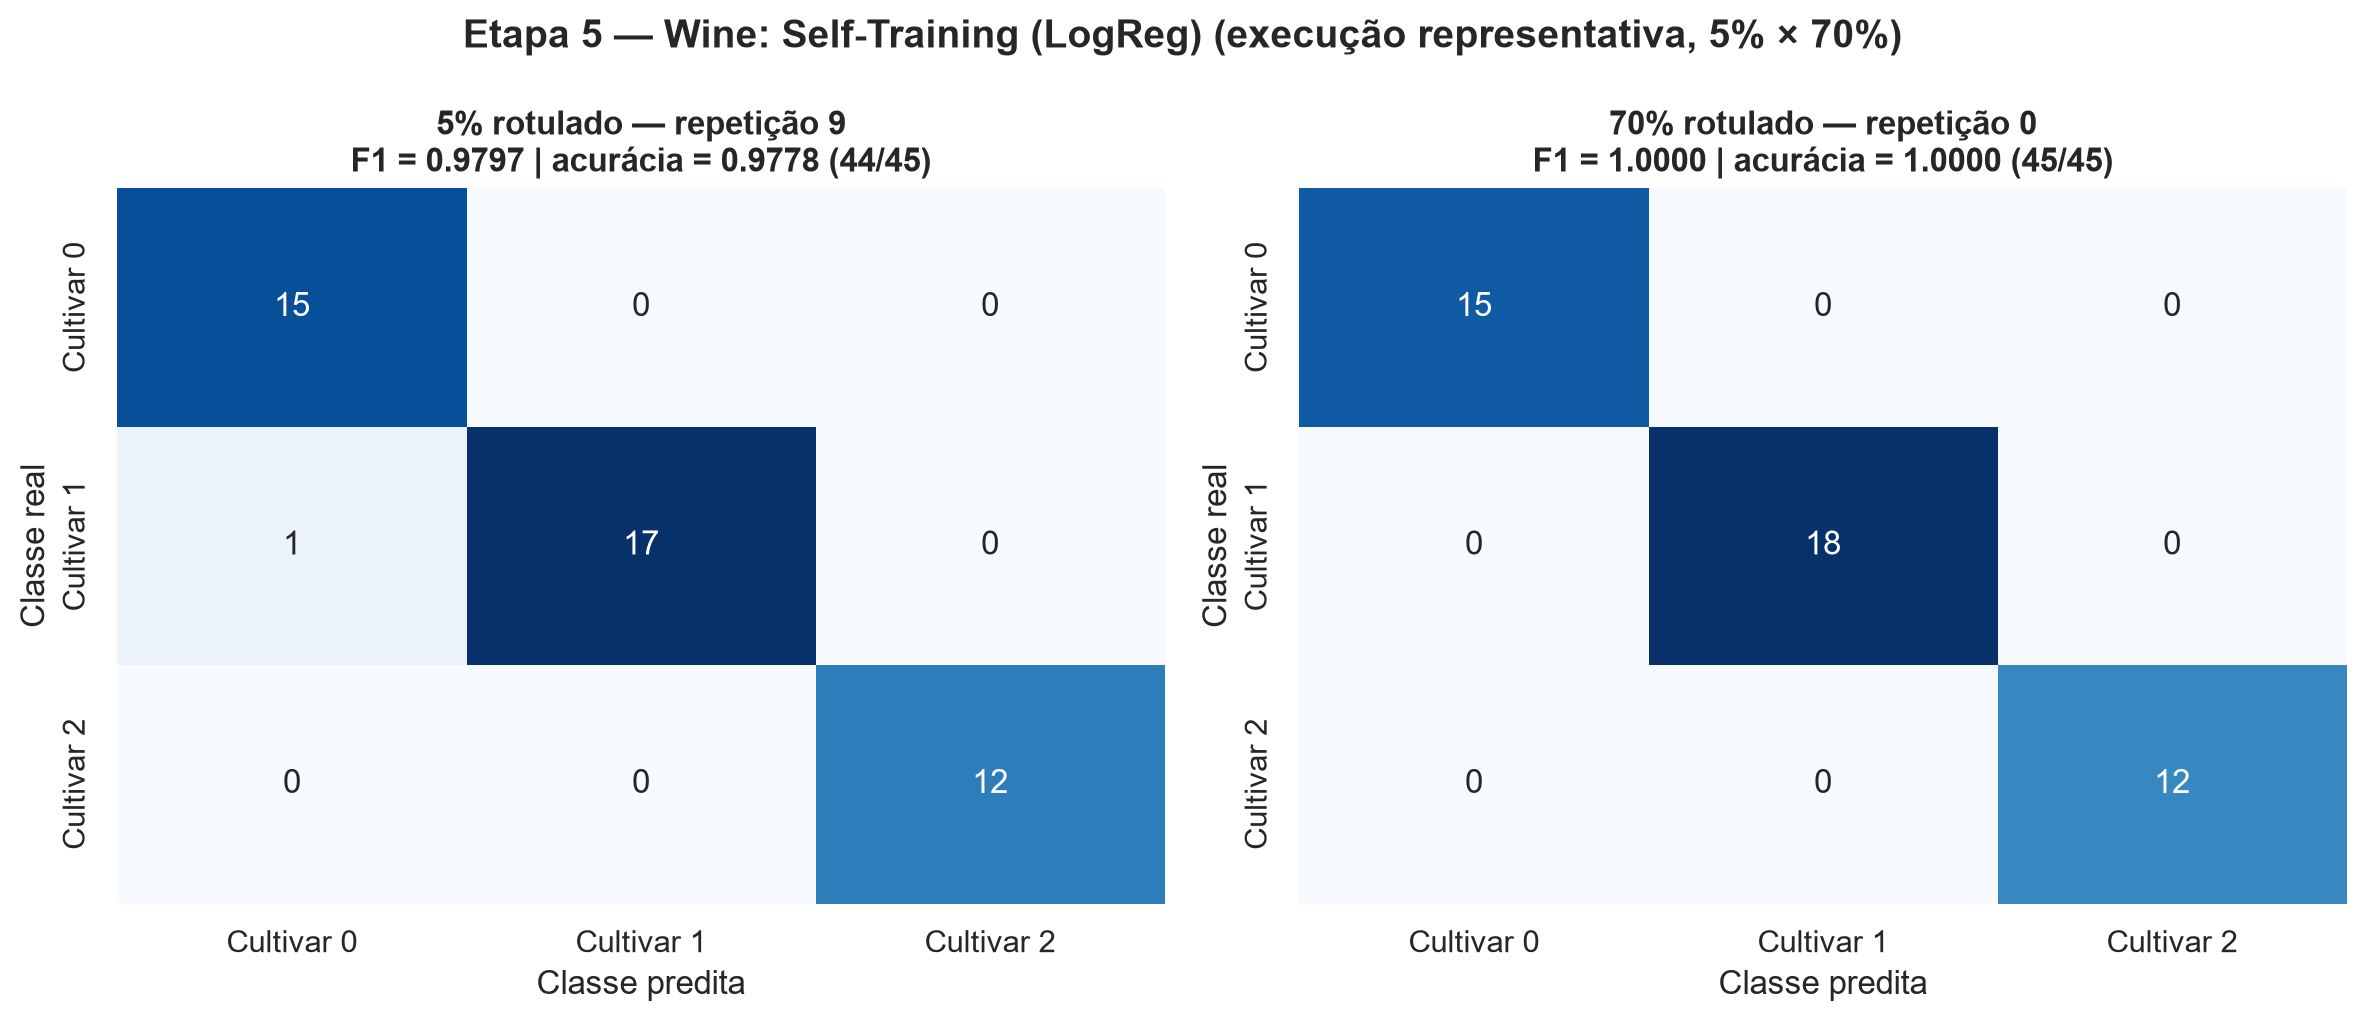
\includegraphics[width=0.9\textwidth, keepaspectratio]{figuras/E5_wine_matriz_representativa.png}
    \caption{Wine: matrizes de confusão do \textit{Self-Training} LR com 5\% e 70\% de rótulos (execuções representativas).}
    \label{fig:matriz_wine}
\end{figure}

No Wine, com 5\% de rótulos, o modelo acerta 44 dos 45 vinhos de teste (97,78\%), com um único erro (um vinho da cultivar 1 classificado como cultivar 0). Com 70\% de rótulos, acerta todos os 45 (100\%). Como o conjunto de teste tem apenas 45 amostras, cada erro corresponde a 2,22 pontos percentuais de acurácia.

\subsection{PROPAGAÇÃO DE RÓTULOS E SENSIBILIDADE AOS HIPERPARÂMETROS}

A Figura \ref{fig:propagacao_wine} ilustra o funcionamento do \textit{Label Spreading} no Wine com 5\% de rótulos: a partir de apenas 7 pontos rotulados, os rótulos são propagados pelo grafo de similaridade para todo o treino, com 86,5\% de acerto nos pontos não rotulados (avaliação transdutiva). Os erros se concentram nas regiões de transição em que a cultivar 1 encosta nas cultivares 0 e 2, e coincidem com os pontos de menor confiança da inferência.

\begin{figure}[htbp]
    \centering
    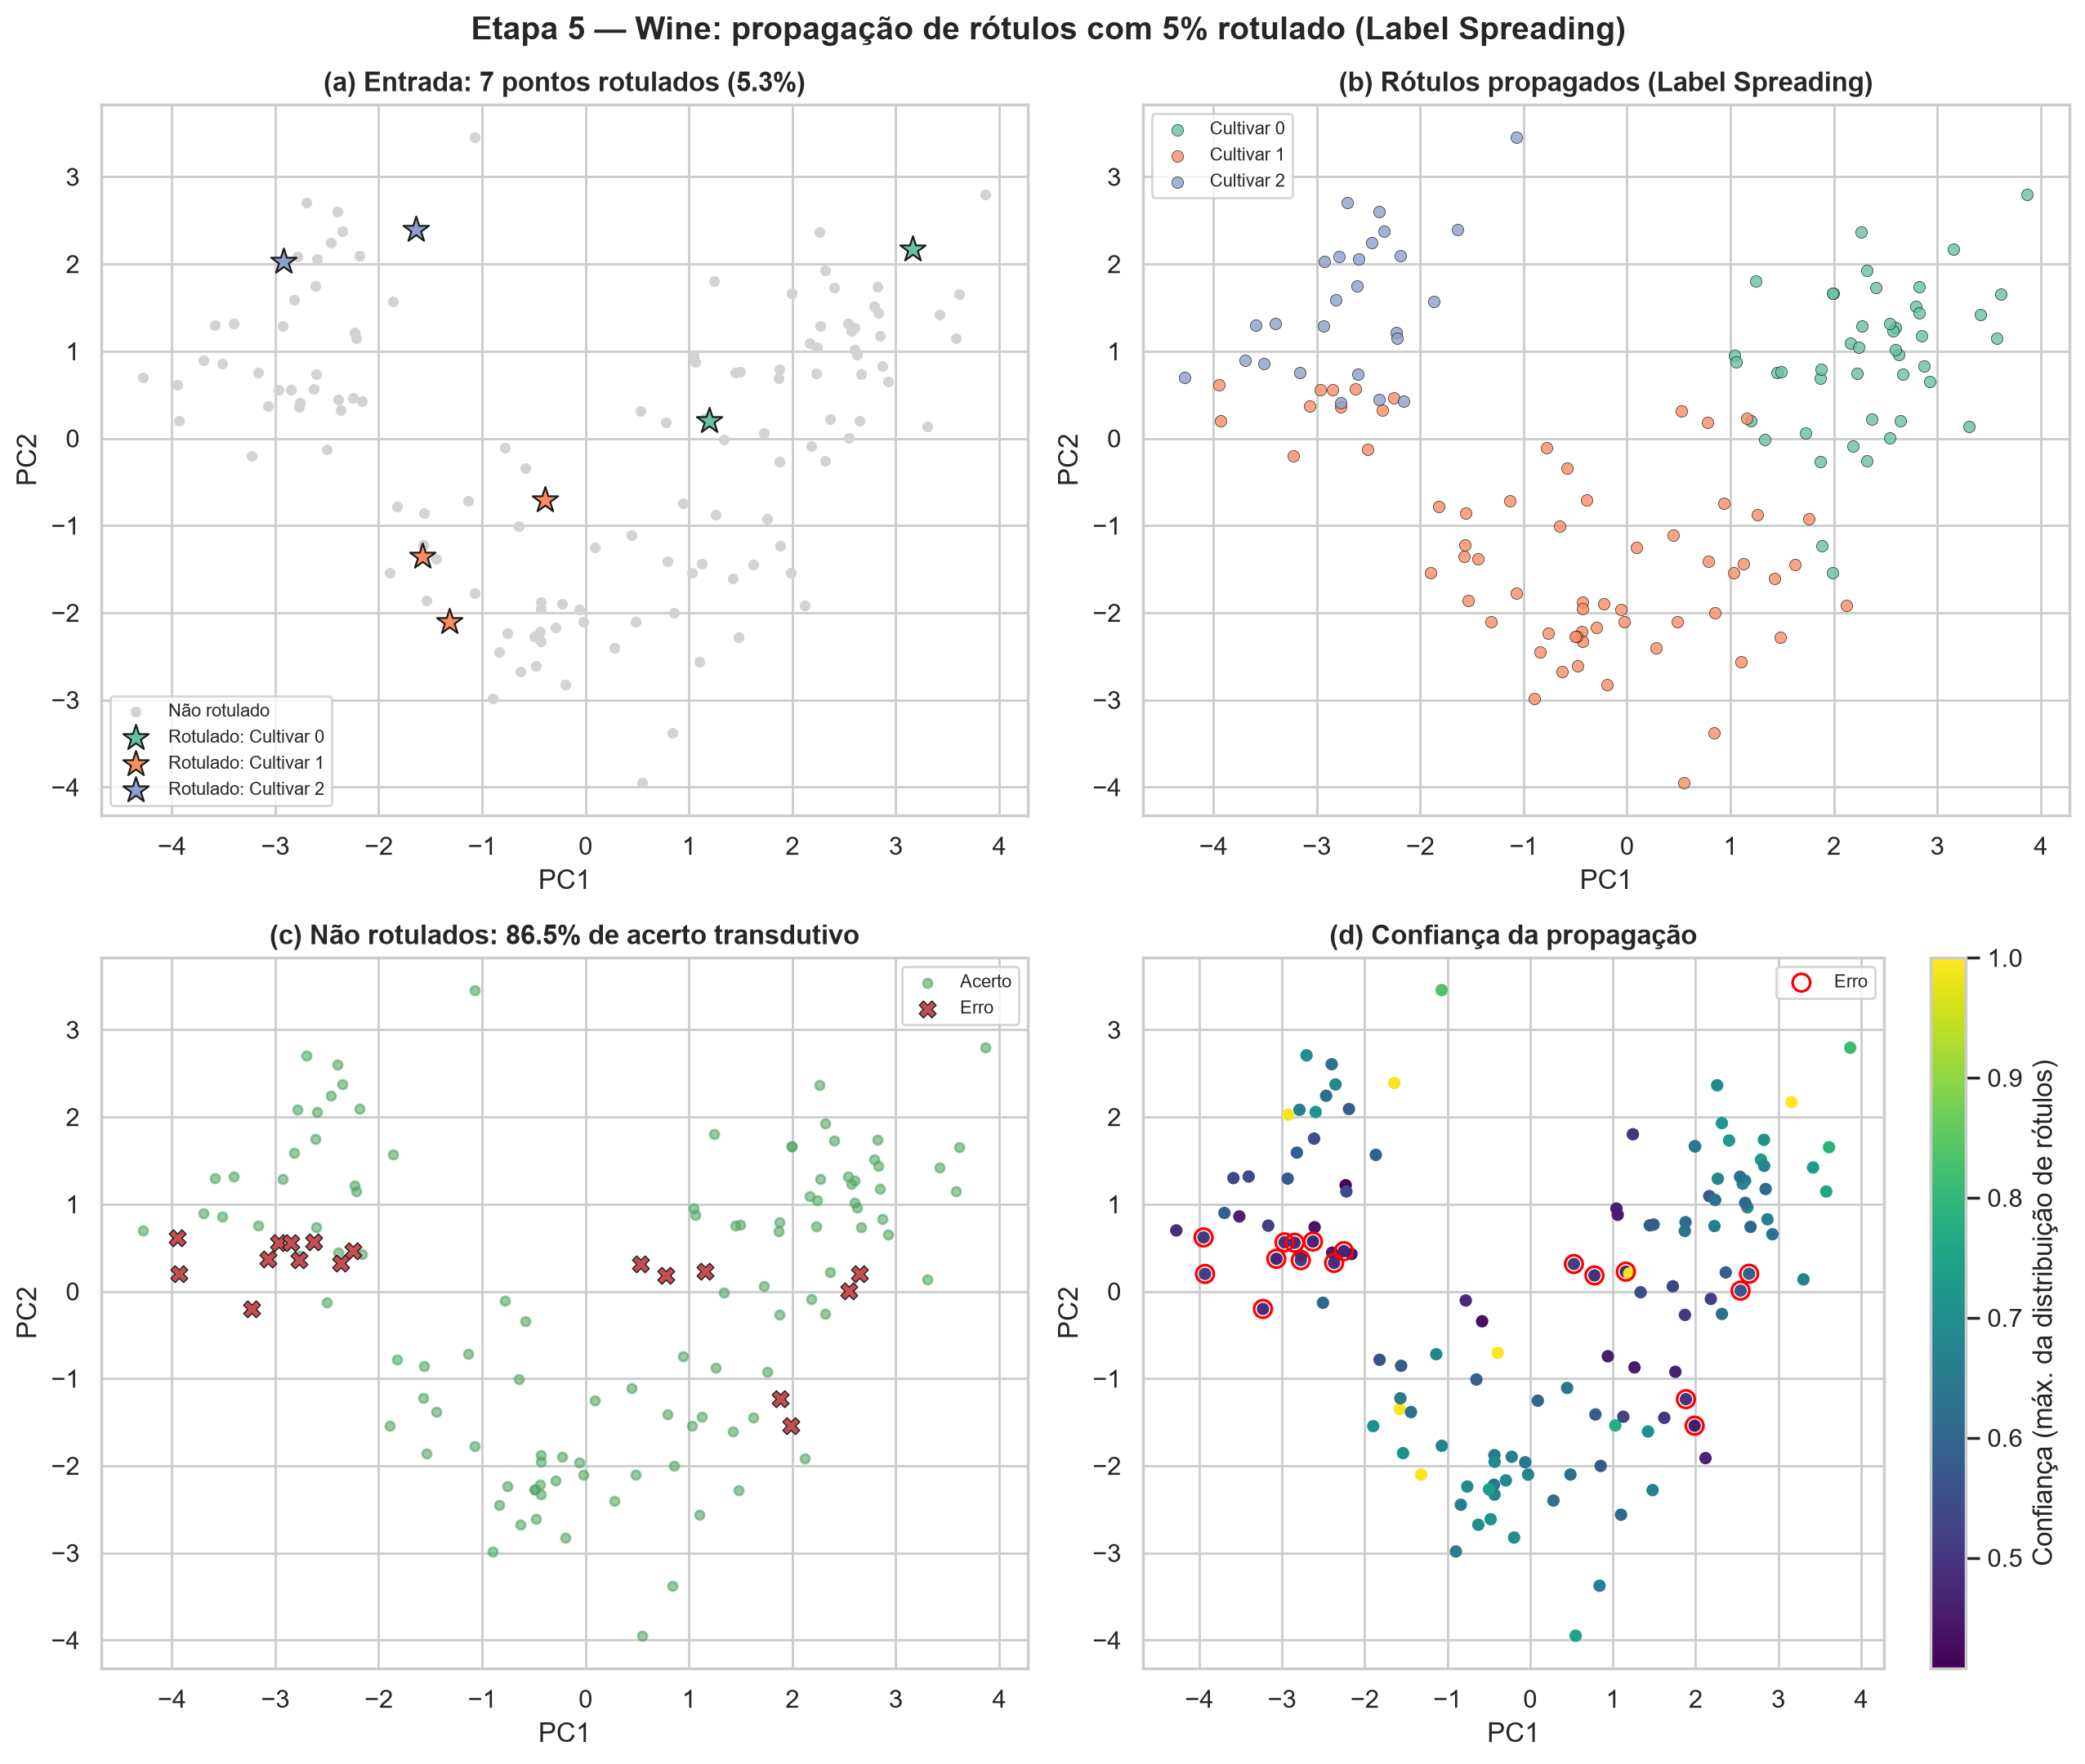
\includegraphics[width=0.85\textwidth, keepaspectratio]{figuras/E5_wine_propagacao_rotulos.png}
    \caption{Wine: \textit{Label Spreading} com 5\% de rótulos no espaço PCA 2D: (a) pontos rotulados, (b) rótulos inferidos, (c) acertos e erros nos não rotulados e (d) confiança da inferência.}
    \label{fig:propagacao_wine}
\end{figure}

Os métodos foram também avaliados variando um hiperparâmetro por vez a partir da configuração dos \textit{scripts}. Os principais achados foram:

\begin{itemize}
    \item \textbf{\textit{Self-Training}} (Figura \ref{fig:sens_self_training}): no Wine com 5\% de rótulos, o limiar de 0,80 faz com que 93,6\% dos pontos não rotulados recebam pseudo-rótulo, com 97,6\% de acerto, levando a F1 = 0,980. Com o limiar de 0,95, apenas 45,2\% são pseudo-rotulados e o F1 cai para 0,855. Com limiares muito altos, quase nada é pseudo-rotulado e o método se reduz à própria Regressão Logística.
    \item \textbf{\textit{Label Spreading} no Wine}: o colapso observado no \textit{Label Propagation} também ocorre no \textit{Label Spreading} quando o núcleo fica largo demais ($\gamma = 0{,}25/13$, F1 = 0,19) ou a suavização forte demais ($\alpha = 0{,}95$, F1 = 0,25). Com $\gamma = 2/13$, por outro lado, o F1 a 5\% chegaria a 0,922.
    \item \textbf{\textit{Label Spreading} no Breast Cancer}: com \texttt{n\_neighbors} = 3, o grafo kNN se fragmenta e 26,6\% dos pontos de teste ficam sem nenhum rótulo alcançável a 5\% (o \texttt{scikit-learn} atribui a eles a classe de índice 0), o que derruba o F1 para 0,758.
    \item \textbf{KNN (\textit{baseline})}: no Wine a 5\%, o \textit{script} usa $k = \min(5, 7/2) = 3$ (F1 = 0,862). Com $k = 5$ e apenas 7 rótulos, o F1 cairia para 0,330, e com $k = 1$ subiria para 0,873. Como as hipóteses comparam sempre com o \textbf{melhor} \textit{baseline} de cada taxa (a Regressão Logística, nesse caso), a escolha de $k$ não infla os ganhos reportados.
\end{itemize}

\begin{figure}[htbp]
    \centering
    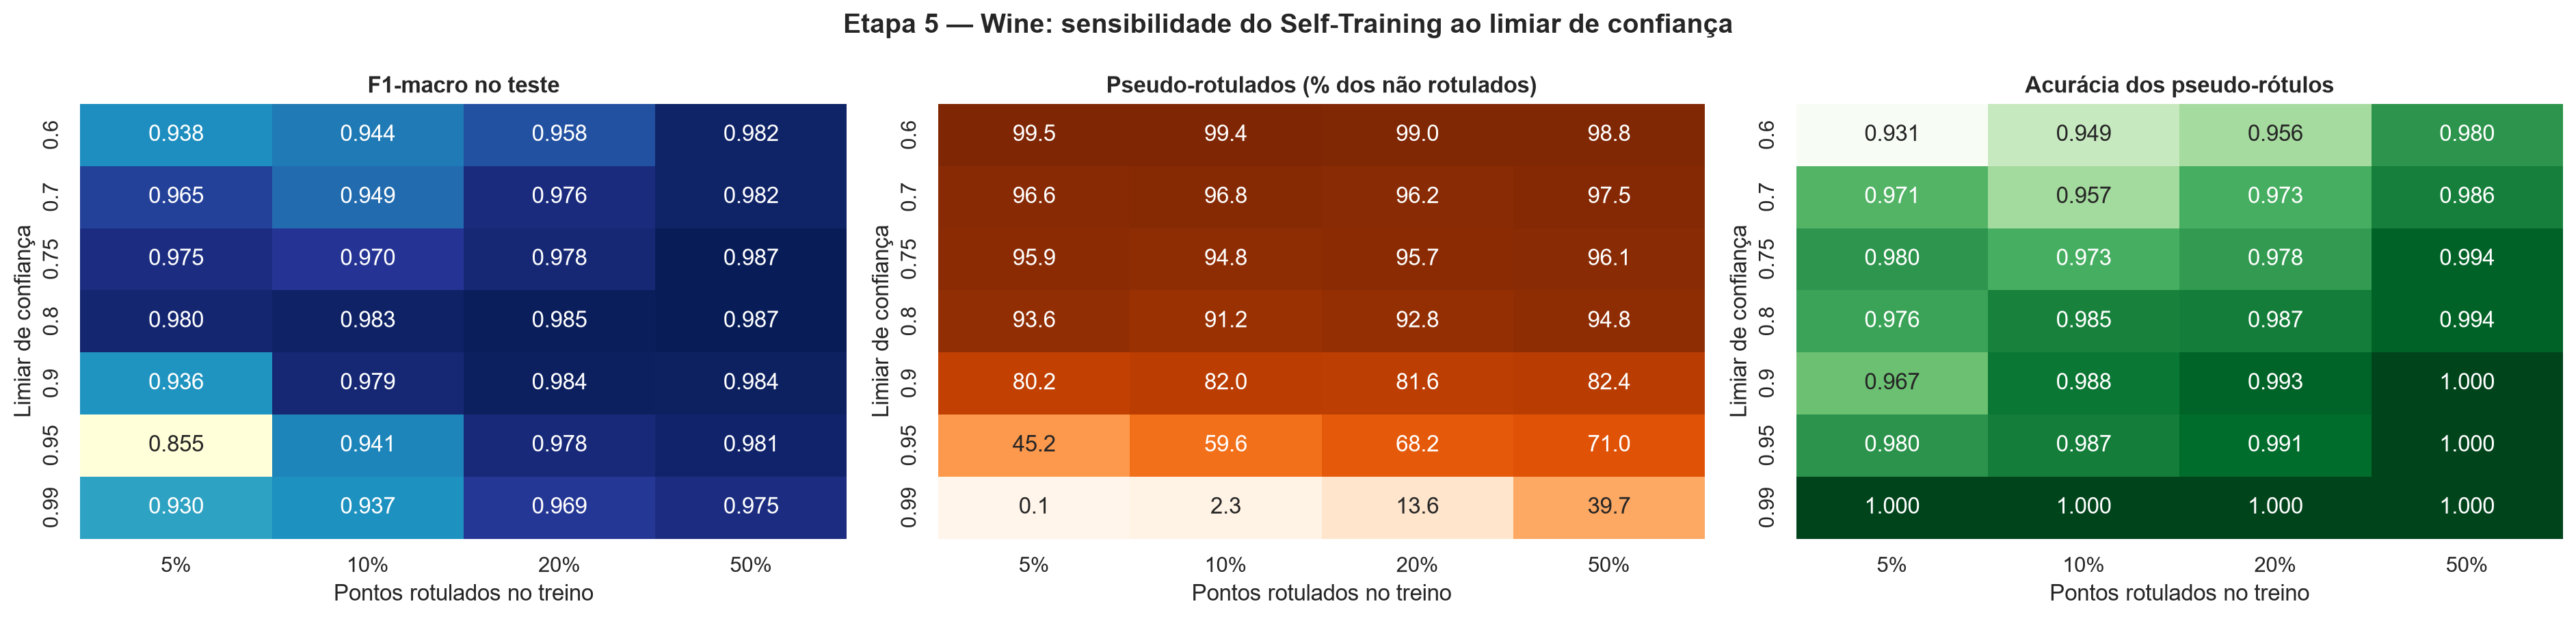
\includegraphics[width=\textwidth, keepaspectratio]{figuras/E5_wine_sensibilidade_self_training.png}
    \caption{Wine: sensibilidade do \textit{Self-Training} ao limiar de confiança: F1-macro no teste, fração de pontos pseudo-rotulados e acurácia dos pseudo-rótulos.}
    \label{fig:sens_self_training}
\end{figure}

Em termos de custo computacional, todos os modelos treinam em milissegundos nessas bases. O \textit{Self-Training} é o mais caro (da ordem de 20 ms, pois retreina a Regressão Logística a cada iteração), e o KNN, o mais barato (menos de 1 ms).
